\documentclass[sigconf,english]{acmart}
\usepackage{demo}
\begin{document}

\setcopyright{acmlicensed}

\copyrightyear{2017} 
\acmYear{2017} 
\setcopyright{rightsretained} 
\acmConference{Programming '17}{April 03-06, 2017}{Brussels, Belgium}
\acmDOI{http://dx.doi.org/10.1145/3079368.3079382}
\acmISBN{978-1-4503-4836-2/17/04}

\title{Tools for open, transparent and engaging storytelling}

\author{Tomas Petricek}
\affiliation{%
  \institution{The Alan Turing Institute}
  \city{London}
  \country{UK}}
\email{tomas@tomasp.net}

\date{5 May 2017}

\begin{abstract}
The rise of Big Data and Open Government Data initiatives means that there is an increasing amount
of raw data about the world available. At the same time, ``post-truth'' has been chosen as the word 
of 2016 \cite{bbc} and the general public increasingly distrusts statistics \cite{guardian}. In 
other words, data science has more capabilities to help us understand the world than ever before, 
yet it is becoming less relevant in public discussion.

This should perhaps not be a surprise as data science is often opaque, non-experts find results 
difficult to interpret and verify, and creating data-driven reports requires advanced skills and 
is limited to a small number of specialists. 

The purpose of the proposed demo is to present The Gamma project (\url{http://thegamma.net}, \cite{dot}) 
which aims to democratize data science. The Gamma encourages everyone -- including journalists and 
interested citizens -- to understand how presented claims are justified, explore data on their own 
and make their own transparent factual claims. If the society is to benefit from the possibilities 
available through data science, it is essential to make data-driven storytelling widely accessible, 
open and engaging.
\end{abstract}


\begin{CCSXML}
<ccs2012>
<concept>
<concept_id>10003120.10003145.10003151.10011771</concept_id>
<concept_desc>Human-centered computing~Visualization toolkits</concept_desc>
<concept_significance>500</concept_significance>
</concept>
<concept>
<concept_id>10011007.10011006.10011008.10011009.10011022</concept_id>
<concept_desc>Software and its engineering~Very high level languages</concept_desc>
<concept_significance>300</concept_significance>
</concept>
</ccs2012>
\end{CCSXML}
\ccsdesc[500]{Human-centered computing~Visualization toolkits}
\ccsdesc[300]{Software and its engineering~Very high level languages}

% Keywords: PLEASE REPLACE
\keywords{Programming experience; example articles}

\maketitle
\section{Open data-driven storytelling}
On one hand, spreadsheets made data exploration accessible to a large number of people, but 
operations performed on spreadsheets are error-prone and cannot be easily reproduced or 
replicated with different data source. On the other hand, data analyses written as programs
can be modified and run repeatedly, but even with the simplest programming tools available, 
building an end-to-end analysis that reads data from a government data source, performs analysis 
and produces an interactive visualization requires expert programming and data science skills.

The Gamma aims to build programming tools that let anyone explore data from a wide range of data 
sources, including open government data, and publish data-driven reports that are:

\begin{itemize}
\item	\textbf{Transparent and accountable}. Readers can review how data is used and discover misleading uses of data.
\item	\textbf{Reproducible and connected}. Readers can run the analysis themselves using the original data source.
\item	\textbf{Open and engaging}. Readers can modify parameters and share reports on different aspects of the data.
\end{itemize}

\noindent
To achieve this, we treat data-driven reports as reproducible programs written in a simple web-based 
scripting language that is integrated with primary data sources (using type providers \cite{inforich,fsdata,idris}) 
and we develop editor tooling that bridges the gap between program-ming and spreadsheets.

\begin{figure*}
\begin{center}
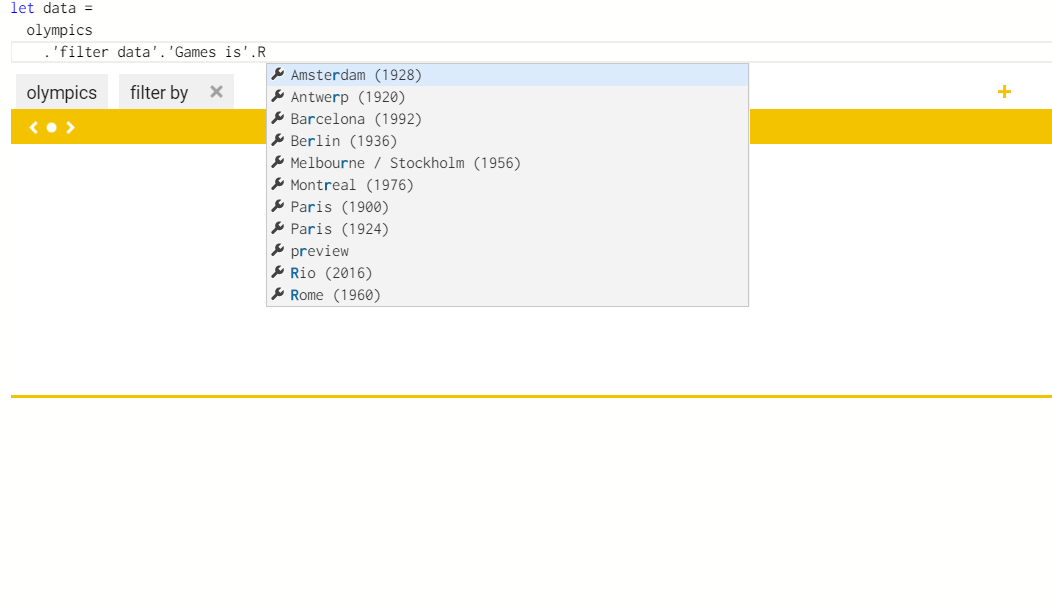
\includegraphics[scale=0.50,trim=0mm 60mm 0mm 0mm,clip]{fig1.png}
\end{center}
\vspace{-2em}
\caption{\textnormal{\small The Gamma project uses a type provider to generate types with members based on the structure 
of the processed data. When writing script to work with data, the auto-completion offers help based 
on the types. In the scripting language behind The Gamma, almost all data processing work is done by 
typing ``.'' and choosing one of the available members, leading to an extremely simple programming model 
that can be well supported by editor tooling.}}
\label{fig1}
\end{figure*}


\begin{figure*}
\begin{center}
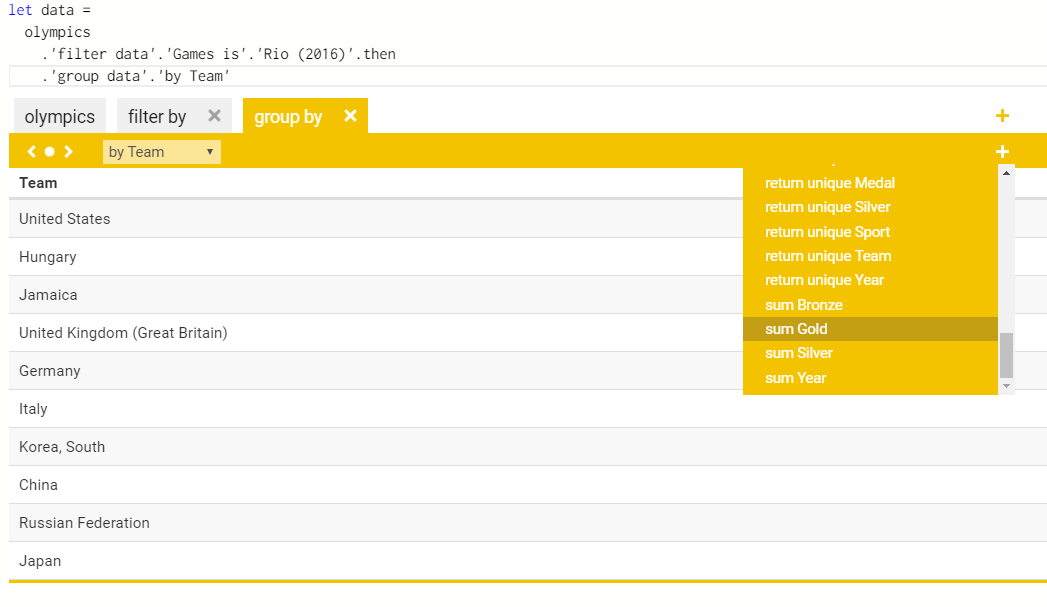
\includegraphics[scale=0.2,trim=0mm 0mm 0mm 0mm,clip]{fig2.png}
\end{center}
\caption{\textnormal{\small When writing data transformations, users can directly edit code that represents the data 
  transformation, but they can also see the preview of the result of the data transformation written
  so far and edit the data transformation in a spreadsheet-inspired manner. Here, the user decided to 
  aggregate data by team (country) and is now choosing aggregations to perform over the group.}}
\label{fig2}
\end{figure*}

\section{Demo outline}
The work presented in the demo session has been focused on building a simple web-based 
library that could be used by data journalists to present visualizations obtained by aggregating and 
summarizing tabular data. Figure~\ref{fig1} and Figure~\ref{fig2} illustrate some of the steps 
performed during a sample task -- given a data table recording individual medals awarded over the 
entire history of the Olympic games, we want to calculate the number of medals per country. 

\section{Innovative aspects of the project}
The project is innovative in two ways. It creates a new simple scripting language for working 
with data and it complements the language with spreadsheet-inspired tooling:

\begin{itemize}
\item \textbf{Simple data-aware language}. When writing code, the programming language understands 
  the data source and data transformations performed so far and offers all available operations when 
  ``.'' is typed. For example, when ``Games is'' is typed in Figure~\ref{fig1}, the editor understands 
  what values are available and offers the user ``Rio (2016)'' in the completion list. This means 
  that the user can construct the whole program just by choosing one of the available operations.
  
\item \textbf{Spreadsheet-inspired editing}. One of the reasons why spreadsheets are easy to use is 
  that the user can always see the data they are working with and manipulate it directly. We adapt 
  this paradigm to programming, taking inspiration from direct-manipulation user interfaces
  \cite{spreadsheetalgebra,querydirect,directman}. In our live editor, the user can always see preview of the 
  aggregation constructed so far, making data exploration easier. As demonstrated in Figure~\ref{fig2}, 
  many transformations can be created using the user interface without writing code directly. 
  Yet, the final result is still an open and reproducible script.
\end{itemize}
  
\noindent
These two innovations make it possible to create web-based data-driven reports that are transparent 
(anyone can see how they are created), open (readers can modify them and share their results) and 
engaging (reader can explore other fun aspects of the data).

The Gamma project is the first step of an increasingly important research that aims to democratize 
data science and encourage every citizen to make factual claims backed by data -- be it for fun or to hold the government accountable.

\begin{acks}
This work was supported by The Alan Turing Institute under the EPSRC grant EP/N510129/1
and by a the Google Digital News Initiative Prototype Fund. 
\end{acks}

\newpage
\nocite{*}

\bibliographystyle{ACM-Reference-Format}
\bibliography{sigproc}
\end{document}
